%% LyX 2.2.0alpha2 created this file.  For more info, see http://www.lyx.org/.
%% Do not edit unless you really know what you are doing.
\documentclass[english]{article}
\usepackage[T1]{fontenc}
\usepackage[latin9]{luainputenc}
\usepackage{geometry}
\geometry{verbose,tmargin=3cm,bmargin=3cm,lmargin=3cm,rmargin=3cm}
\usepackage{units}
\usepackage{amsmath}
\usepackage{graphicx}
\usepackage{esint}

\makeatletter
%%%%%%%%%%%%%%%%%%%%%%%%%%%%%% Textclass specific LaTeX commands.
\newenvironment{lyxcode}
{\par\begin{list}{}{
\setlength{\rightmargin}{\leftmargin}
\setlength{\listparindent}{0pt}% needed for AMS classes
\raggedright
\setlength{\itemsep}{0pt}
\setlength{\parsep}{0pt}
\normalfont\ttfamily}%
 \item[]}
{\end{list}}

%%%%%%%%%%%%%%%%%%%%%%%%%%%%%% User specified LaTeX commands.
\usepackage{fancyheadings}
\pagestyle{fancy}
\lhead{Kellen Betts}
\chead{imageCorrectionLinearDiffusion}
\rhead{160731}

\makeatother

\usepackage{babel}
\begin{document}

\title{Image Correction with Linear and Diffusion Filtering}

\author{Kellen Betts}

\date{Updated July 31, 2016}
\maketitle
\begin{abstract}
In this project corrupted images of male supermodel Derek Zoolander
are received, and two image processing techniques are implemented
to repair the images. The techniques are used for both color and black
and white images. Linear filtering is used to denoise a set of images
that are corrupted by noise across the entire image. Using both a
Gaussian and Shannon filter, moderate success is achieved. A diffusion
process is then developed to restore a second set of images that contain
noise confined to a small region. The localized nature of the corruption
and spatial flexibility of the diffusion process result is near perfect
restoration for the second set of images. Finally, a combination of
linear filtering and diffusion is explored as a hybrid method for
the first images, but only minimal improvement over the individual
methods is observed.
\end{abstract}

\section{Introduction}

The setup for this project involves two sets of images (Figure 1)
of the fictional male supermodel Derek Zoolander that have been corrupted
by protestors. One set of images contains noise across the entire
image, and one set is corrupted in a localized region near Derek's
nose. The first objective (Task 1) is to repair the images with global
noise using a linear filter. Both a Gaussian and Shannon filter will
be tested. The next objective (Task 2) is to use a diffusion process
to repair the images with noise confined to a small region since diffusion
is effective when targeting specific regions of an image. Finally,
diffusion and linear filtering are compared and their combination
is explored as a hybrid method to achieve better results.

\begin{lyxcode}
\noindent \begin{center}
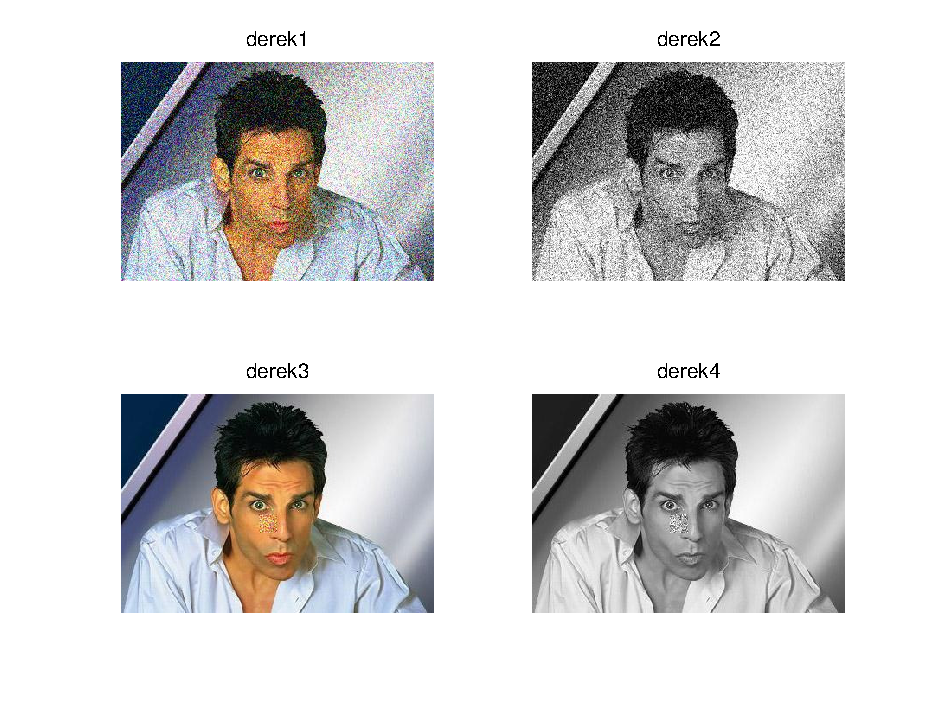
\includegraphics[width=0.55\columnwidth]{plots/originals}~\\
\textbf{}%
\begin{minipage}[t]{0.6\columnwidth}%
\textbf{Figure 1.} Original corrupted images received for the project.%
\end{minipage}
\par\end{center}
\pagebreak{}
\end{lyxcode}

\section{Theoretical Background}

Linear filtering of images is similar to time-frequency analysis in
that the spectral component of data, in this case of an image, is
used to apply a linear filter to remove specific frequency components.
The basis for the frequency transformation used in this method is
the Fourier Transform. For a given function $f(x)$ the transform
and its inverse are defined,
\begin{equation}
F\left(k\right)=\frac{1}{\sqrt{2\pi}}\intop_{-\infty}^{\infty}e^{-ikx}f\left(x\right)dx
\end{equation}
\begin{equation}
f(x)=\frac{1}{\sqrt{2\pi}}\intop_{-\infty}^{\infty}e^{ikx}F(k)dk
\end{equation}
where $k$ corresponds to the wave-numbers in the trigonometric identity.
With the Fourier transform, the image data is integrated over the
domain $x\,\epsilon\,\left[-\infty,\infty\right]$ resolving the frequency
content. Computationally the transform is implemented over a finite
domain $x\,\epsilon\,\left[-L,L\right]$ using the Fast Fourier Transform
(FFT). One of the important advantages of the FFT algorithm is the
low operation count of $O\left(N\,\log N\right)$ using a $2^{n}$
discritization. Additionally, given its trigonometric construction,
the transform assumes a $2\pi$-periodic domain.

Many different linear filters can be used in image processing. In
this project the noise in the image data is shown to be high frequency,
so one filter used is a Gaussian (Kutz 13.2.57),
\begin{equation}
F\left(k_{x},k_{y}\right)=\exp\left(-\sigma_{x}\left(k_{x}-a\right)^{2}-\sigma_{y}\left(k_{y}-b\right)^{2}\right)
\end{equation}
centered at $\left(a,b\right)$ with filter widths $\sigma_{x}$ and
$\sigma_{y}$ . Another filter used is a Shannon based on the step
function,
\begin{equation}
F_{A}\left(x,y\right)=\begin{cases}
1 & if\,x,y\,\epsilon\,A\\
0 & if\,x,y\,\notin\,A
\end{cases}
\end{equation}
where $A$ is a targeted area of specified dimensions.

The second method used to remove the noise from image data is diffusion.
The use of diffusion can be shown to be equivalent to linear filtering
with a Gaussian function by considering a general diffusion equation
(Kutz 13.3.58),
\begin{equation}
u_{t}=D\nabla^{2}u
\end{equation}
where $D$ is a diffusion coefficient, $u\equiv u\left(x,y\right)$,
and the Laplacian $\nabla^{2}=\partial_{x}^{2}+\partial_{y}^{2}$
. If periodic boundaries are assumed, $\left(5\right)$ can be solved
using the Fourier transform giving (Kutz 13.3.59),
\begin{equation}
\hat{u_{t}}=-D\left(k_{x}^{2}+k_{y}^{2}\right)\hat{u}\quad\rightarrow\quad\hat{u}=\hat{u_{0}}\,\exp\left(-D\left(k_{x}^{2}+k_{y}^{2}\right)t\right)
\end{equation}
which shows that the linear Gaussian filter $\left(3\right)$ is equivalent
to the solution $\left(6\right)$ of the general diffusion equation
$\left(5\right)$. To implement this method computationally, $\left(5\right)$
can be rewritten (Kutz 13.3.60),
\begin{equation}
u_{t}=\nabla\cdot\left(D(x,y\right)\nabla u
\end{equation}
where $D\left(x,y\right)$ is a spatial diffusion coefficient that
will be used to apply the method on images with a finite region of
noise. This differential equation $\left(7\right)$ can be discritized
using a second-order center difference scheme where the $x$-domain
is (Kutz 13.3.61a),
\begin{equation}
\frac{\partial^{2}u}{\partial x^{2}}=\frac{1}{\triangle x^{2}}\left[u\left(x+\triangle x,\,y\right)-2u\left(x,\,y\right)+u\left(x-\triangle x,\,y\right)\right]
\end{equation}
and a similar scheme is used for $\nicefrac{\partial^{2}u}{\partial y^{2}}$.
The discritized linear system for $\left(7\right)$ in one dimension
is given by (Kutz 13.3.63),
\begin{equation}
\frac{d\mathbf{u}}{dt}=\frac{k}{\triangle x^{2}}\mathbf{Au}
\end{equation}
where the second-order center difference scheme $\left(8\right)$
with periodic boundaries gives the Laplacian operator (Kutz 13.3.64),
\begin{equation}
\mathbf{A}=\begin{bmatrix}-2 & 1 & 0 & \cdots & 0 & 1\\
1 & -2 & 1 & 0 &  & 0\\
0 & \ddots & \ddots & \ddots &  & \vdots\\
\vdots &  &  &  &  & 0\\
0 &  & 0 & 1 & -2 & 1\\
1 & 0 & \cdots & 0 & 1 & -2
\end{bmatrix}
\end{equation}
To denoise images in a finite region, diffusion is localized by defining
the spatial coefficient $D\left(x,y\right)$ using a smooth Gaussian
similar to the linear filter $\left(3\right)$ with, 
\begin{equation}
D\left(x,y\right)=C\,\exp\left(-\sigma_{x}\left(x-a\right)^{2}-\sigma_{y}\left(y-b\right)^{2}\right)
\end{equation}
which is centered at $\left(a,b\right)$ with the constant $C$ and
widths $\sigma_{x}$ and $\sigma_{y}$ . 

\section{Algorithm Implementation and Development}

\subsection*{Image Import/Plotting:}

The JPG images are imported using the $\mathtt{imread}$ command.
The incoming data is in 8-bit integer format, so it is converted to
double before any further operations are performed. Black and white
images import as a $x\times y\times1$ grid, and color images as $x\times y\times3$
corresponding to the rgb color profile. Each color channel is processed
separately, then stitched back together at the end. Plotting of images
is done using the $\mathtt{imshow}$ command requiring conversion
back to 8-bit integer format. Several independent plotting functions
are developed (see Appendix B) which greatly simplifies the plot code
needed to output the results from the various filtering and diffusion
processes.

\subsection*{Linear Filtering:}

There are four basic steps in the linear filtering procedure:
\begin{enumerate}
\item Importing images and initializing vectors/parameters.
\item Transforming image data into frequency domain using FFT.
\item Applying Gaussian or Shannon filter function.
\item Inverse transform of the filtered data back to spatial domain.
\end{enumerate}
The flow of operations is controlled by a main script $\mathtt{hw3\_task1.m}$
. The images are 253x361 so the $x,y$ domain does not match the $2^{n}$
discritization necessary to achieve minimum operation count with the
FFT. The closest $2^{n}$ discritization is $2^{8}\times2^{9}=256\times512$
and so rescaling would require significant extrapolation. 

The primary filtering operations are run in a separate function $\mathtt{hw3\_filter.m}$
so that exploration of optimal parameters can be automated. In the
function, the frequency domain is discritized $1:x_{n}$ and $1:y_{n}$
because the filter is applied to frequency data that is shifted back
to the linear discritization. 1D wave-number vectors are transformed
to 2D grids using the $\mathtt{meshgrid}$ command. The Gaussian filter
is calculated using,
\[
\mathtt{F=exp(-sigma(k)*(Kx-(w/2+1)).^{2}-sigma(k)*(Ky-(h/2+1)).^{2})}
\]
where the sigma and center parameters are explored extensively to
achieve best results. A Shannon filter centered at $\left(a,b\right)$
is implemented using,
\[
\mathtt{F(b-width:1:b+width,a-width:1:a+width)=1}
\]
with the remaining regions of $F$ filled with zeros and width parameter
explored until best results are achieved. 

The 2D image data (individual color channel if rgb) is transformed
and shifted in frequency domain using the $\mathtt{fft2}$ and $\mathtt{fftshift}$
commands respectively. The frequency data is then multiplied by the
specified filter. Finally, the data is inverse shifted/transformed
and returned to the main script for plotting and analysis.

\subsection*{Diffusion:}

There are four basic steps in the diffusion procedure:
\begin{enumerate}
\item Import of images and initialization of vectors/parameters.
\item Building a sparse 2D differentiation matrix $\left(L\right)$.
\item Building a sparse coefficient matrix $D\left(x,y\right)$ for localized
diffusion.
\item Solving the linear system with the ODE solver.
\end{enumerate}
The flow of operations is controlled by a main script $\mathtt{hw3\_task2.m}$,
with primary operations run in the separate function $\mathtt{hw3\_diffusion.m}$.
The spatial domains $\left(x,y\right)$ are linearly discritized.
Sparse derivative matrices are built using the $\mathtt{spdiags}$
command for each 1D domain $\left(x,y\right)$ corresponding to the
$A$ matrix $\left(10\right)$. The 1D operators are then stitched
together to make a sparse 2D Laplacian operator $\left(L\right)$
using the $\mathtt{kron}$ command.

For diffusion applied to a localized region, the sparse coefficient
matrix $D\left(x,y\right)$ is built using the $\mathtt{spdiags}$
command as well. The matrix is discritized using a smooth Gaussian
function,
\[
\mathtt{D2(jx,jy)=C*D2(jx,jy)*exp(-sigma*(jx-a).^{2}-sigma*(jy-b).^{2})}
\]
which gives the diffusion operation spatial localization centered
at $\left(a,b\right)$. The sigma and center $\left(a,b\right)$ parameters
are explored extensively to achieve best results.

Next, the 2D image data (individual color channel if rgb) is passed
to the ODE solver $\mathtt{ode113}$ (see Appendix A) with the 2D
Laplacian operator $\left(L\right)$, coefficient matrix $D\left(x,y\right)$,
and parameters for the time interval steps. The ODE solver calls a
separate function $\mathtt{hw3\_rhs.m}$ which contains the right-hand-side
operation of the linear system,
\[
\mathtt{rhs=coeff*L*u}
\]
Having multi-channel data (rgb color) means output from the ODE solver
has to be handled carefully to ensure images are stitched back together
correctly.

\section{Computational Results}

\subsection*{Task 1:}

The objective in Task 1 is to repair the set of images (Figure 2)
with global noise using a linear filter. The images both appear to
have similar noise across the entire image. Visualizing the frequency
component of the image on a log scale (Figure 3, left) clearly shows
frequencies in the unfiltered image are concentrated at low frequencies,
so the objective is to remove the effects of high-frequency noise.

\pagebreak{}

\begin{lyxcode}
\noindent \begin{center}
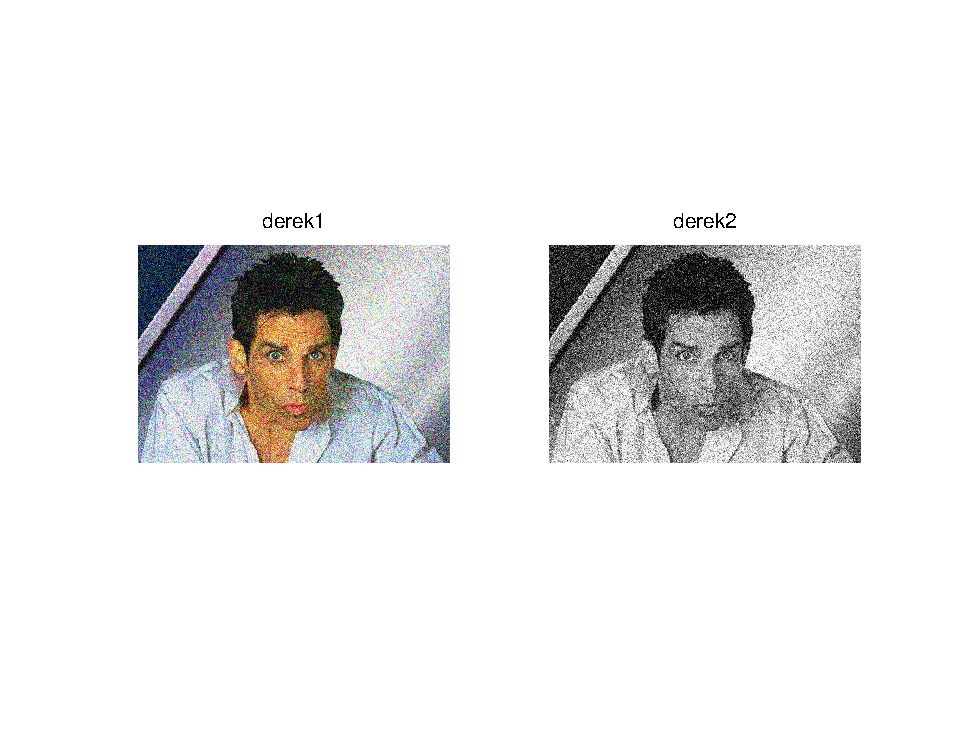
\includegraphics[width=0.75\columnwidth]{plots/task1_originals}\textbf{}~\\
\textbf{}%
\begin{minipage}[t]{0.75\columnwidth}%
\textbf{Figure 2.} Original images showing noise corruption across
the entire $x,y$ spatial domain.%
\end{minipage}
\par\end{center}
\noindent \begin{center}
\vspace{0.04\paperheight}
\par\end{center}

\end{lyxcode}
For the Gaussian filter, different values of the width parameter were
explored (Figure 4) with a value $\sigma\approx0.0025$ showing the
best balance of noise reduction and blur. The frequency plot for the
filtered image (Figure 3, right) shows that the Gaussian filter with
$\sigma=0.0025$ spreads the distribution. When processing the images,
each channel is isolated and filtered separately (Figure 5). The best
results achieved for the Gaussian filter with both the color and black
and white images are seen in Figure 6. These images indicate the Gaussian
filter is able to moderately reduce the noise in the original images
with slight image blur.

\begin{lyxcode}
\noindent \begin{center}
\vspace{0.02\paperheight}
\par\end{center}
\noindent \begin{center}
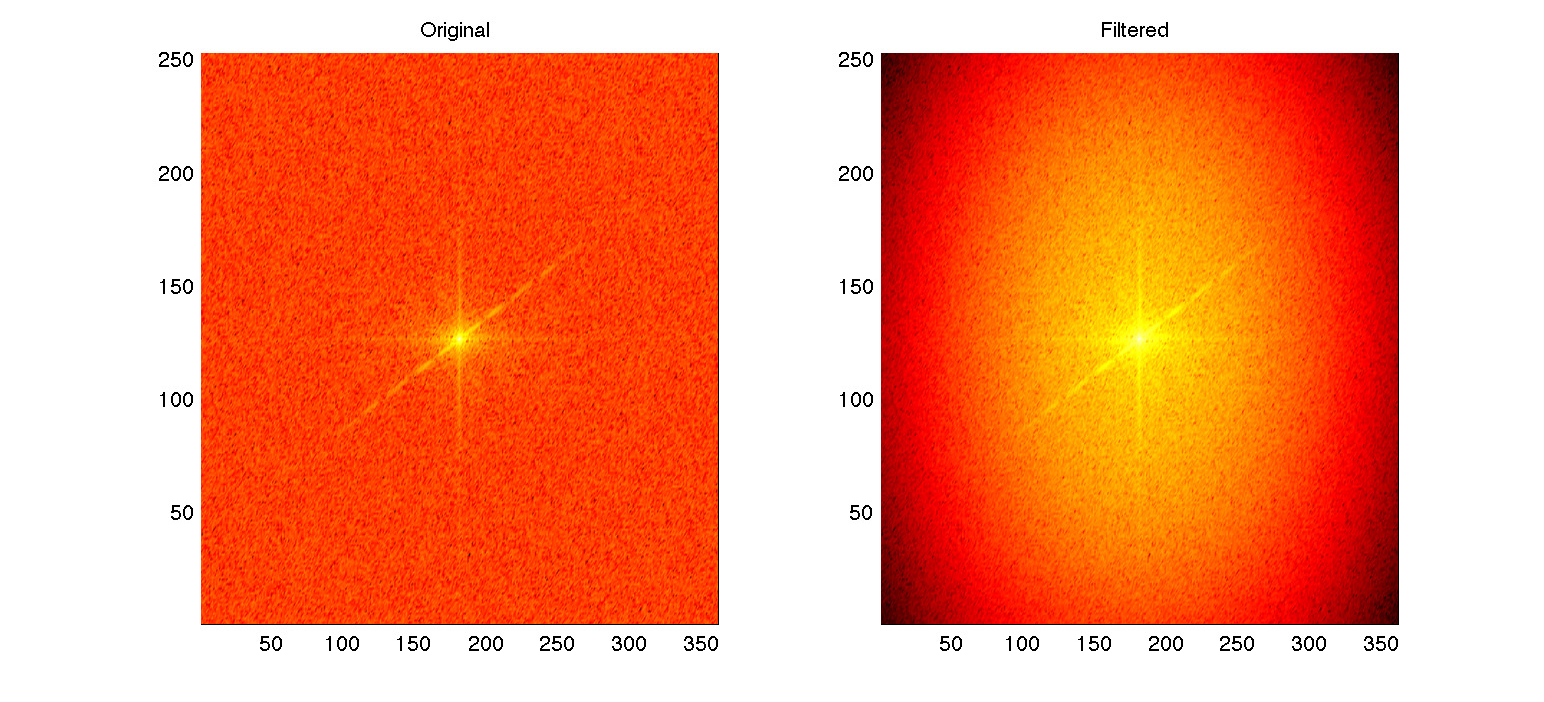
\includegraphics[width=0.75\columnwidth]{plots/task1_transform_gauss}\textbf{}~\\
\textbf{}%
\begin{minipage}[t]{0.75\columnwidth}%
\textbf{Figure 3.} Comparison of the log of the Fourier transform
for the original noisy image (left) and Gaussian filtered with $\sigma=0.0025$
(right). The filter appears to improve the frequency distribution
moderately. %
\end{minipage}
\par\end{center}
\pagebreak{}
\noindent \begin{center}
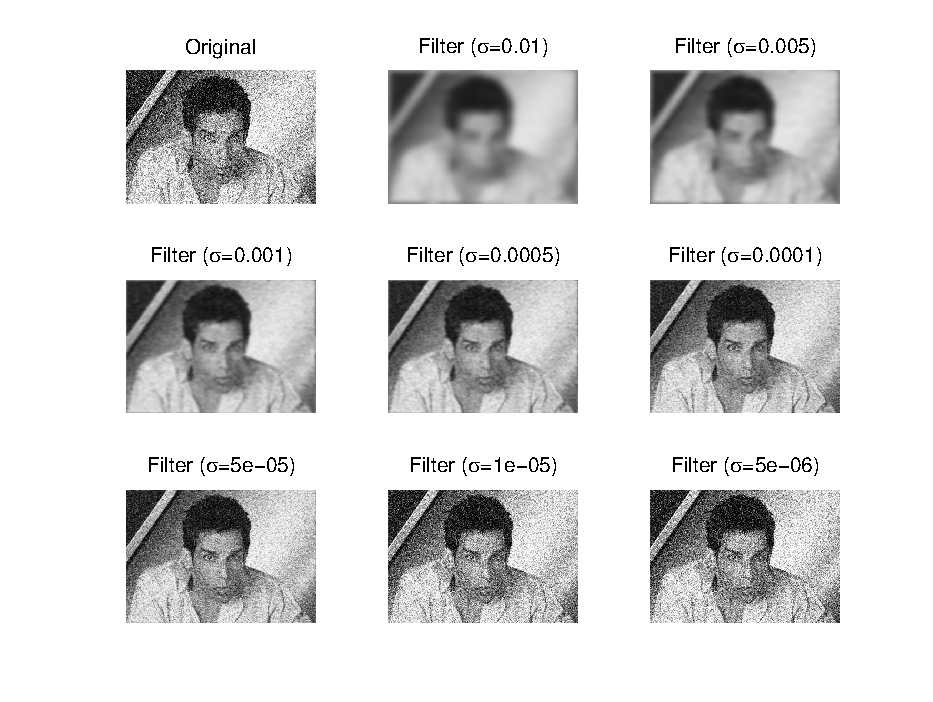
\includegraphics[width=0.75\columnwidth]{plots/task1_sigSeries1}\textbf{}~\\
\textbf{}%
\begin{minipage}[t]{0.75\columnwidth}%
\textbf{Figure 4.} Series of images exploring Gaussian filter width
$\left(\sigma\right)$ values. The optimal value at $\sigma\approx0.0025$
best balances the tradeoff between noise reduction and blurring.%
\end{minipage}
\par\end{center}
\noindent \begin{center}
\par\end{center}
\noindent \begin{center}
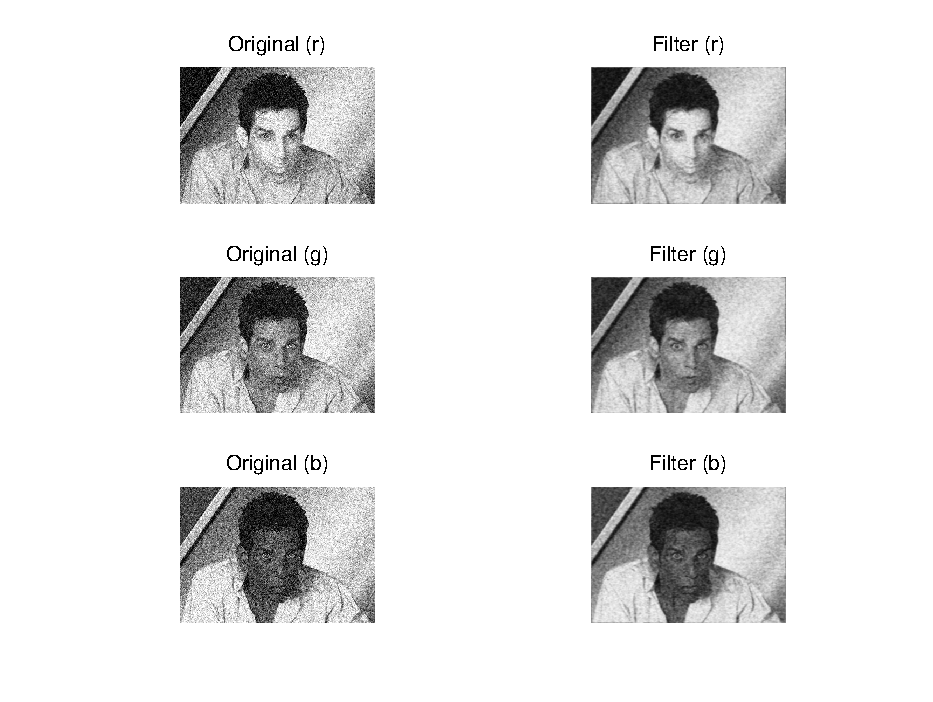
\includegraphics[width=0.75\columnwidth]{plots/task1_filter_color}\textbf{}~\\
\textbf{}%
\begin{minipage}[t]{0.75\columnwidth}%
\textbf{Figure 5.} The Gaussian filter $\left(\sigma=0.0025\right)$
is applied separately for each channel of the color image. The channels
are then stitched back together to build a filter color image.%
\end{minipage}
\par\end{center}
\pagebreak{}

\noindent \begin{center}
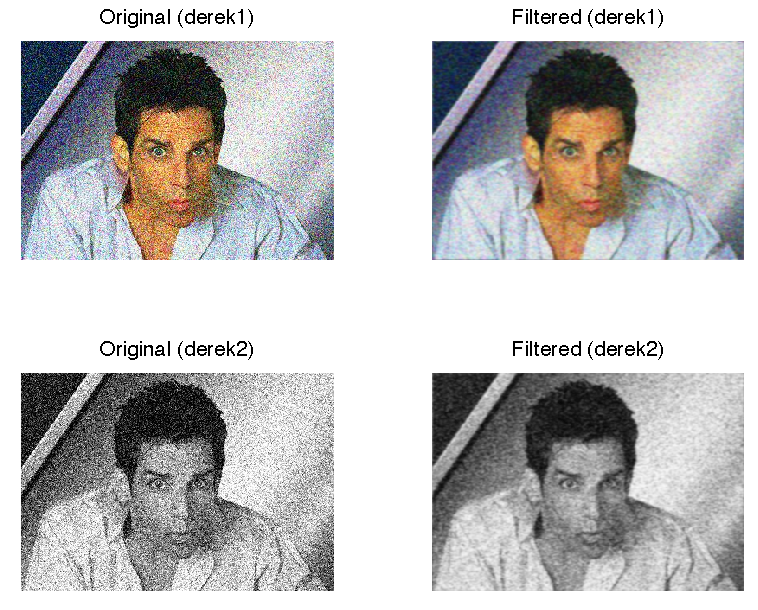
\includegraphics[width=0.65\columnwidth]{plots/task1_result_gauss}\textbf{}~\\
\textbf{}%
\begin{minipage}[t]{0.75\columnwidth}%
\textbf{Figure 6.} Comparison of the original noisy image (left) with
the best results achieved for the Gaussian filter (right) with $\sigma=0.0025$.
The filter appears to moderately remove the noise in the image while
slightly reducing image sharpness.%
\end{minipage}
\par\end{center}
\noindent \begin{center}
\vspace{0.005\paperheight}
\par\end{center}

\end{lyxcode}
For the Shannon filter, testing different values of the width parameter
shows that a width of 50 pixels has the best balance of noise reduction
and blur. The effect of the Shannon filter on the frequency distribution
is seen in Figure 7 (right), where all frequencies that fall outside
the window are zeroed out. Figure 8 shows the best results for both
the Gaussian and Shannon filters. The results indicate that both filters
moderately removed the noise corrupting the images. The Shannon filter
appears to better preserve the sharpness of the image, which agrees
with its step-function construction. Conversely, the smoothly varying
Gaussian appears to remove more noise (it can reach inside the Shannon
window), but also slightly reduces image sharpness meaning some necessary
frequency content is lost.

\begin{lyxcode}
\noindent \begin{center}
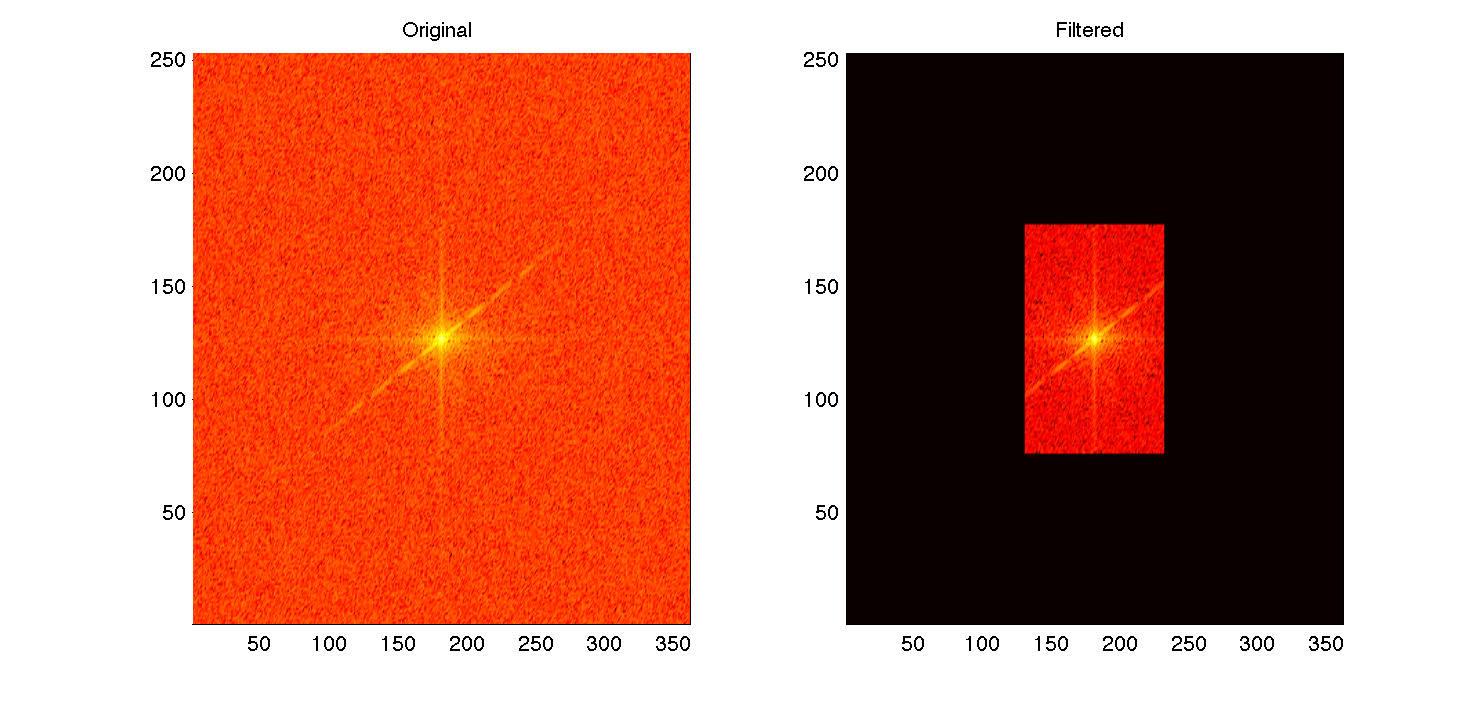
\includegraphics[width=0.75\columnwidth]{plots/task1_transform_shan}\textbf{}~\\
\textbf{}%
\begin{minipage}[t]{0.75\columnwidth}%
\textbf{Figure 7.} Comparison of the log of the Fourier transform
for the original noisy image (left) and Shannon filtered with a window
width of 50 pixels (right).%
\end{minipage}
\par\end{center}
\pagebreak{}

\noindent \begin{center}
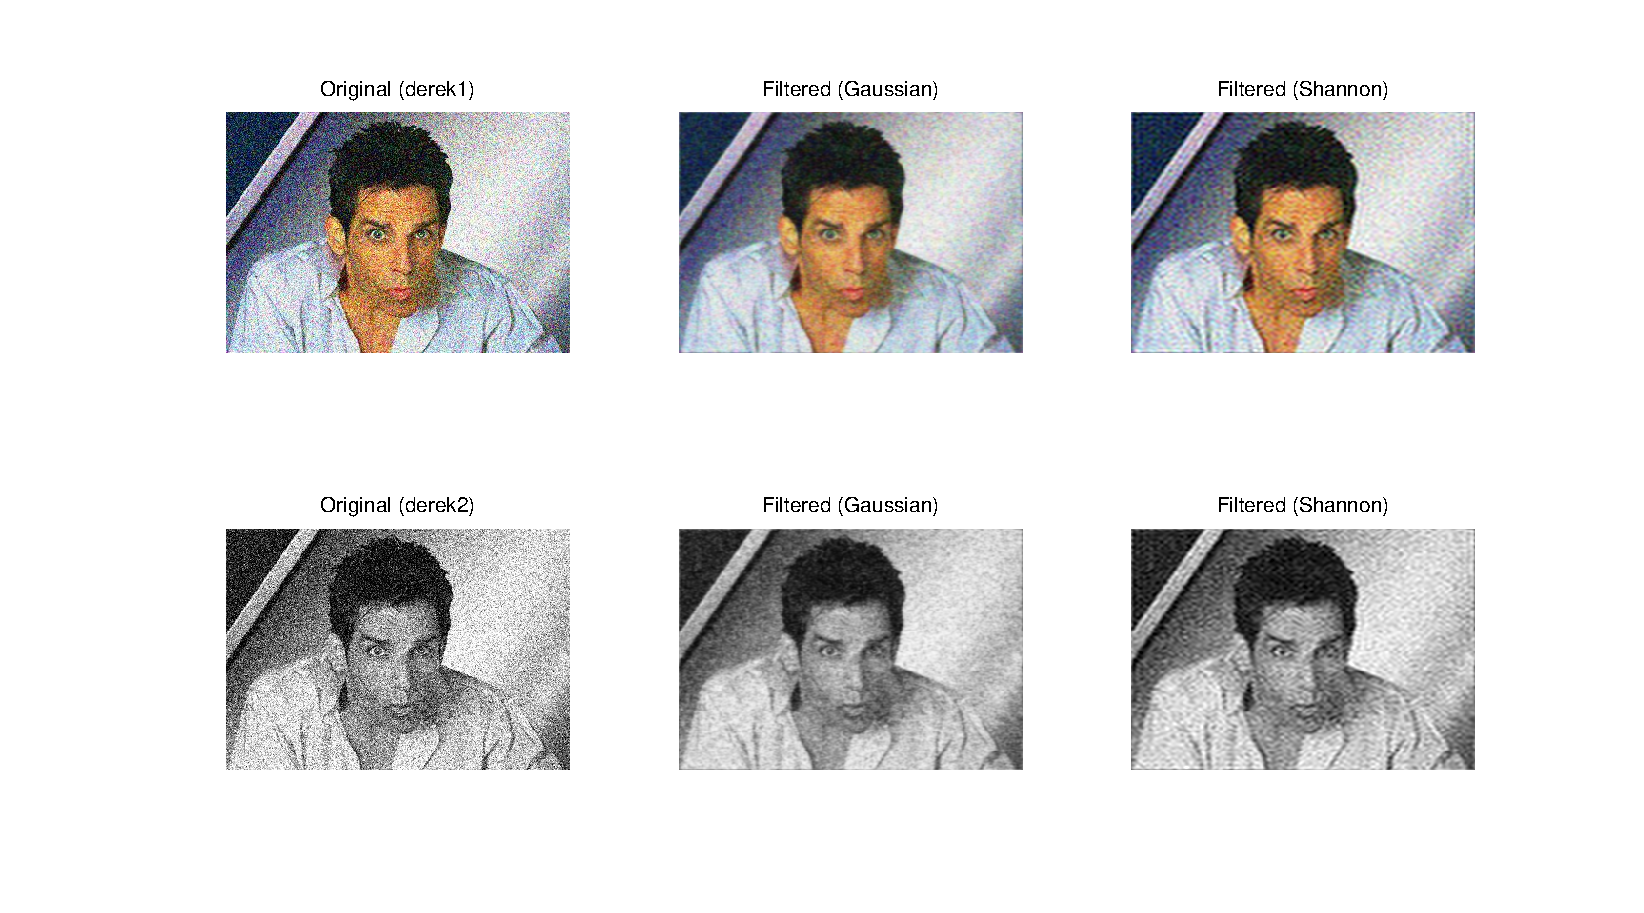
\includegraphics[width=0.85\columnwidth]{plots/task1_comparison}\textbf{}~\\
\textbf{}%
\begin{minipage}[t]{0.75\columnwidth}%
\textbf{Figure 8.} Comparison of the original noisy image (left) with
the best results for the Gaussian filter (center) with $\sigma=0.0025$
and the Shannon filter (right) with a width of 50px. The Shannon filter
appears to better preserve the sharpness of the image, while the Gaussian
appears to remove more noise but also slightly reduce image sharpness.%
\end{minipage}
\par\end{center}

\end{lyxcode}
\noindent \begin{center}
\vspace{0.005\paperheight}
\par\end{center}

\subsection*{Task 2:}

The objective of Task 2 is to repair a set of images (Figure 9) with
noise corruption localized to a small square region. Both images appear
to have the same corruption. The noise patch in the images appears
slightly lower and left of image center, so the $\left(a,b\right)$
coordinates were iterated starting from image center until the optimal
coordinates $\left(155,162\right)$ were determined. The time interval
parameter is extensively explored, and as seen in Figure 10 a value
of $t\approx0.03$ best balances the tradeoff between removal of the
local noise and preservation of adjacent image detail. For the black
and white images, a slight higher value $\left(t\approx0.05\right)$
is optimal. The best results achieved for denoising with the diffusion
process (Figure 11) show the noise patch is effectively removed with
minimal disturbance to adjacent detail. Since the patch is removed
with the diffusion process, additional filtering is unnecessary.
\begin{lyxcode}

\noindent \begin{center}
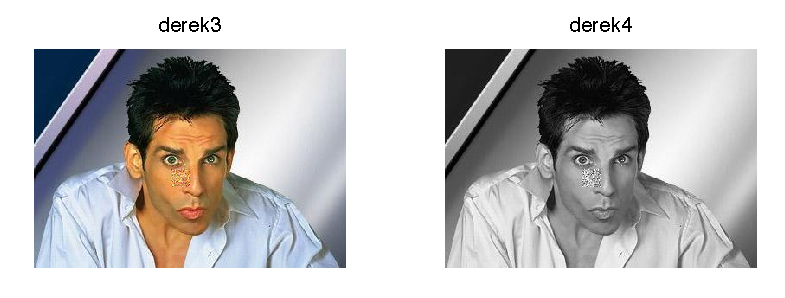
\includegraphics[width=0.75\columnwidth]{plots/task2_originals}\textbf{}~\\
\textbf{}%
\begin{minipage}[t]{0.75\columnwidth}%
\textbf{Figure 9.} Original images showing noise corruption localized
to a square region near the nose.%
\end{minipage}
\par\end{center}
\pagebreak{}
\noindent \begin{center}
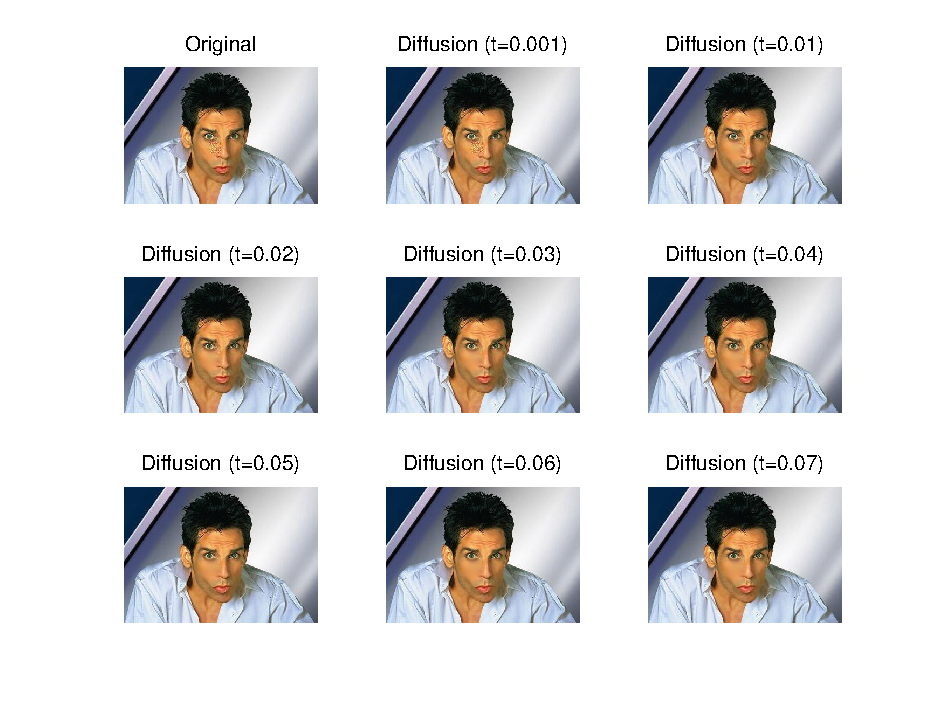
\includegraphics[width=0.75\columnwidth]{plots/task2_color_series}\textbf{}~\\
\textbf{}%
\begin{minipage}[t]{0.75\columnwidth}%
\textbf{Figure 10.} Series exploring time interval parameter. The
value at $t\approx0.03$ best balances the tradeoff between removal
of the local noise and preservation of adjacent image detail.%
\end{minipage}
\par\end{center}

\noindent \begin{center}
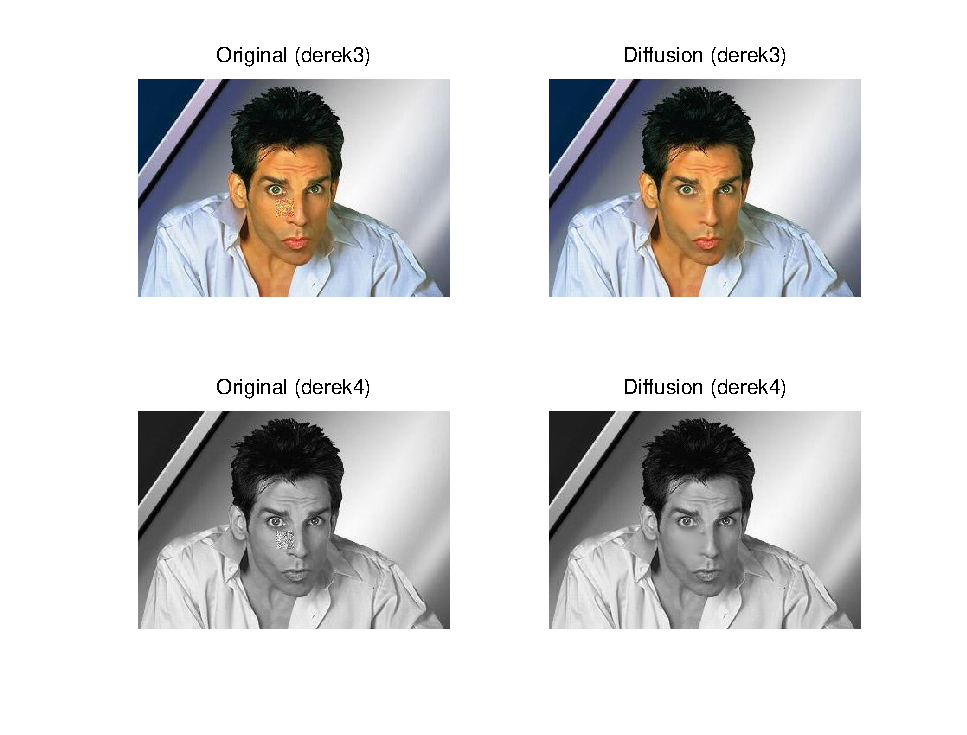
\includegraphics[width=0.75\columnwidth]{plots/task2_result}\textbf{}~\\
\textbf{}%
\begin{minipage}[t]{0.75\columnwidth}%
\textbf{Figure 11.} Comparison of the original (left) with localize
noise patch and the best result for denoising with the diffusion process
(right). These show the noise patch is effectively removed with minimal
disturbance to adjacent detail.%
\end{minipage}
\par\end{center}
\pagebreak{}
\end{lyxcode}

\subsection*{Additional Tests:}

Using the techniques developed in Task 1 and Task 2, the diffusion
and filtering processes can be further explored by applying diffusion
to the images from Task 1 and comparing the results with the filters.
First, the diffusion process is optimized for the images from Task
1 using a constant coefficient $D$ since the targeted spatial region
is the entire image and testing the time interval parameter. The optimal
values for these images are $D=0.005$ at $t\approx0.01$ which best
balances the tradeoff between removal noise and loss of image sharpness.
Comparison (Figure 12) of the diffusion process at $t=0.01$ with
the Gaussian and Shannon filters shows that diffusion achieves similar
results with a moderate reduction in noise. This is not surprising
since the linear Gaussian filter $\left(3\right)$ and Fourier solution
to the diffusion equation $\left(6\right)$ are shown to be equivalent
(see section 2).

Finally, sequential denoising techniques with both filtering and diffusion
are tested using the techniques and parameters previously established.
If the original noisy images are filtered using the Gaussian then
subsequently sent through the diffusion process (Figure 13), only
moderate improvement in the final image quality is seen. Similar results
are seen if the sequence is reversed with diffusion applied first
(Figure 14).

\noindent \begin{center}
\vspace{0.05\paperheight}
\par\end{center}
\begin{lyxcode}
\noindent \begin{center}
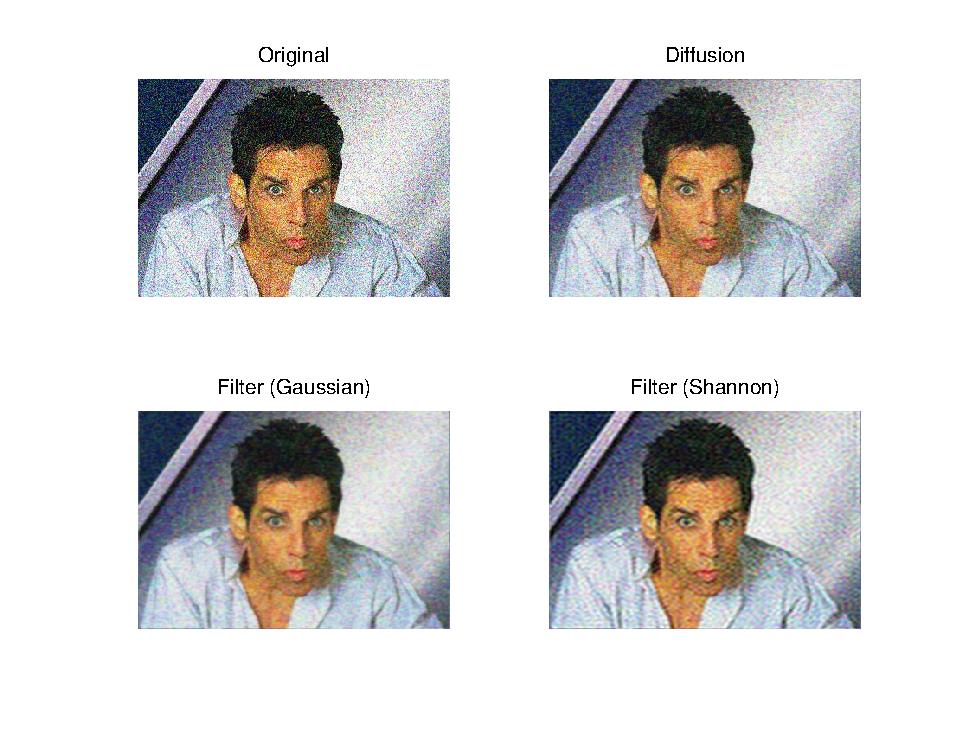
\includegraphics[width=0.85\columnwidth]{plots/versus}\textbf{}~\\
\textbf{}%
\begin{minipage}[t]{0.75\columnwidth}%
\textbf{Figure 12.} Comparison of the original noisy image (upper
left) with denoising by diffusion (upper right), Gaussian filter (lower
left), and Shannon filter (lower right). Diffusion is similar to both
filter methods, falling in the middle for the tradeoff of noise removal
and image sharpness.%
\end{minipage}
\par\end{center}
\pagebreak{}
\end{lyxcode}
\noindent \begin{center}
\vspace{0.01\paperheight}
\par\end{center}
\begin{lyxcode}
\noindent \begin{center}
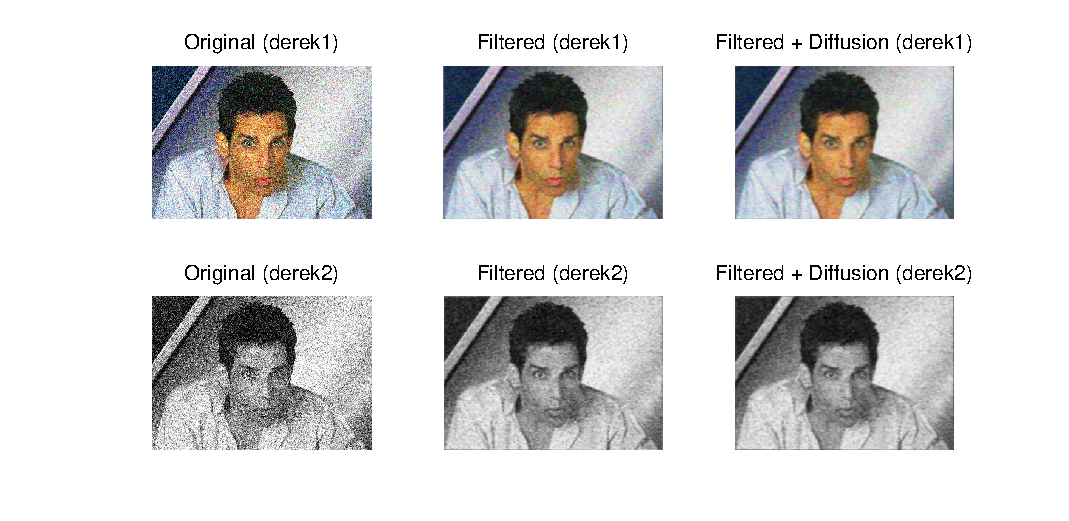
\includegraphics[width=0.85\columnwidth]{plots/hybrid_filtFirst}\textbf{}~\\
\textbf{}%
\begin{minipage}[t]{0.75\columnwidth}%
\textbf{Figure 13.} Comparison of the original noisy image (left)
with the results from the Gaussian filter (center) and a sequential
denoising by diffusion (right). Moderate improvement in image quality
is achieved with this technique.%
\end{minipage}
\par\end{center}

\end{lyxcode}
\noindent \begin{center}
\vspace{0.05\paperheight}
\par\end{center}
\begin{lyxcode}

\noindent \begin{center}
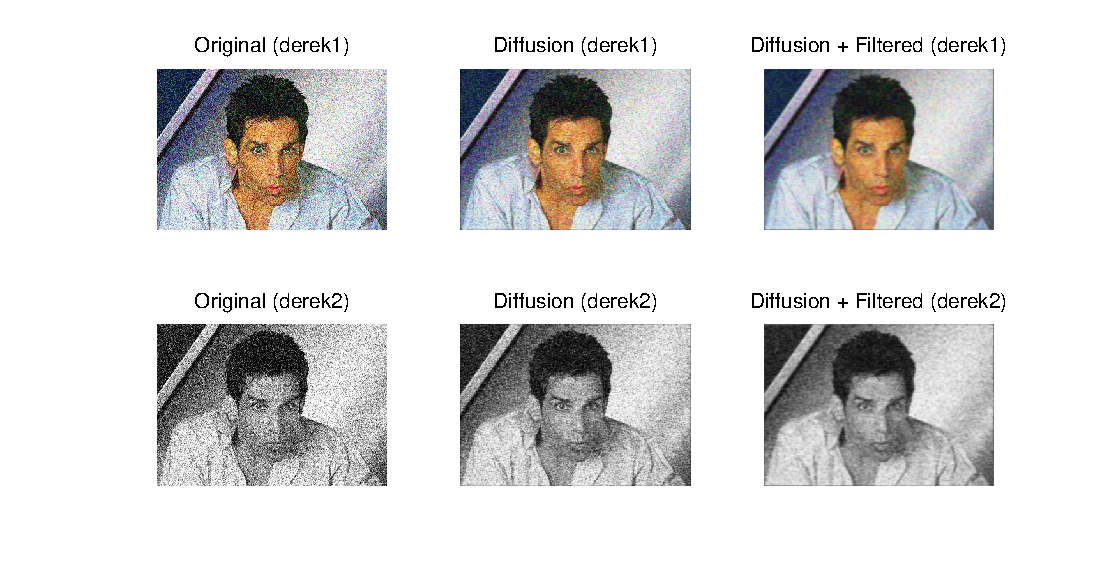
\includegraphics[width=0.85\columnwidth]{plots/hybrid_diffFirst}\textbf{}~\\
\textbf{}%
\begin{minipage}[t]{0.75\columnwidth}%
\textbf{Figure 14.} Comparison of the original noisy image (left)
with the results from denoising by diffusion (center) and sequential
Gaussian filter (right). Moderate improvement in image quality is
achieved with this technique as well.%
\end{minipage}
\par\end{center}
\pagebreak{}
\end{lyxcode}

\section{Summary and Conclusions}

Ultimately, in this project image processing techniques, including
linear filtering and diffusion, are developed and applied to two sets
of images corrupted by noise. One set is corrupted by noise across
the entire image, and linear filtering with both Gaussian and Shannon
filters are shown to have moderate success. The second set of images
has a patch of noise localized to a small square region. These images
are repaired using a diffusion process with a targeted spatial coefficient
matrix. The results show that diffusion is highly effective at removing
the localized noise, but when it applied to the images with noise
across the entire image the results are comparable to linear filtering.
Additionally, hybrid techniques with both linear filtering and diffusion
show minimal improvement. 

One of the more substantial challenges faced in this project was building
the targeted coefficient matrix for the diffusion process. The initial
version I made caused matrix multiplication errors when used in the
rhs function. Fortunately, one of my classmates provided a suggestion
on the discussion board that resolved the dimensioning problem I was
having, and I am indebted to their contribution. 

\section*{Appendix A}

\subsubsection*{MATLAB commands used:}
\begin{description}
\item [{abs}] Takes the absolute value.
\item [{ceil}] Used to round an operation toward $\infty$.
\item [{eye}] Builds identity matrices for given dimension. Used when building
1D derivative matrices and 2D Laplacian operator.
\item [{fftn}] The all important FFT function, which performs a discritized
Fourier Transforms. This version of the function transforms $n$-dimensional
data. The $\mathtt{fft}$ and $\mathtt{fft}2$ versions transform
1- and 2-dimensional data respectively.
\item [{fftshift}] The output of the $\mathtt{fft}$ algorithm is shifted
(butterfly algorithm), so data in the frequency domain is shifted
back using this function before plotting.
\item [{imread}] Load the data in an image file into a matrix that can
then be used for subsequent data manipulations.
\item [{imshow}] Used to plot image data.
\item [{kron}] Builds a large matrix filled with all possible element-wise
products for given matrices. Used to build the 2D l=Laplacian operator
from 1D derivative matrices.
\item [{load}] Loads data from an external file.
\item [{length}] Used to get the length of vectors.
\item [{linspace}] Used to build a linear vector with $n+1$ points for
the spatial domain. The vector is then trimmed to $n$ points due
to the periodic boundaries.
\item [{meshgrid}] Transforms the domain of given vector input to multi-dimension
matrices.
\item [{nextpow2}] Used to find the next power of 2 for a given input.
Since FFT is optimal with a $2^{n}$ discritization, the datasets
are trimmed to a $2^{n}$ length.
\item [{num2str}] Used to convert a number to a string.
\item [{ode113}] Non-stiff ODE solver use for time evolution of linear
system. Has a default relative tolerance of $10^{-3}$ and absolute
tolerance of $10^{-6}$.
\item [{ones}] Used to build vector/matrices pre-filled with ``1''.
\item [{pcolor}] Used to plot the 3D spectrograms.
\item [{plot}] Used to plot the various parameters agains time or frequency.
\item [{real}] Returns $\mathrm{Re}\left(z\right)$ for a given input.
\item [{reshape}] Reshapes vector or matrix for given dimensions.
\item [{spdiags}] Builds sparse diagonal matrices from given vector and
indices. This is a critical tool for lower operation count when solving
linear systems.
\item [{strcat}] Used to concatenate a string.
\item [{subplot}] Used to produce plot arrays.
\item [{switch}] Condition structure used to vary code execution based
on a specified tag.
\item [{tic/toc}] Used to time the operations.
\item [{uint8}] Used to convert data to 8-bit integer format.
\item [{zeros}] Used to build vectors and matrices filled with ``0''.
\end{description}

\section*{Appendix B}

See the project root for files.

\subsection*{Task 1:}

Main control script $\mathtt{task1.m}$ and linear filtering function
$\mathtt{filter.m}$.

\subsection*{Task 2:}

Main control script $\mathtt{task2.m}$, diffusion filtering function
$\mathtt{diffusion.m}$ and right-hand-side function $\mathtt{rhs.m}$.

\subsection*{Plotting and related:}
\begin{itemize}
\item $\mathtt{plot\_imgPick.m}$
\item $\mathtt{plot\_array22.m}$ (note: $\mathtt{plot\_array23.m}$ is
essentially identical but plots a 2x3 subplot array)
\item $\mathtt{plot\_diffSeries.m}$
\item $\mathtt{plot\_filtered.m}$
\item $\mathtt{plot\_fourier.m}$
\end{itemize}

\end{document}
